\chapter{Introduzione}
\label{sec:intro}


\section[Programmazione su GPU]{Programmazione su GPU}

Sin dalla nascita delle prime \gls{CPU}, l'obiettivo principale degli ingegneri è stato quello di aumentare le prestazioni dei processori. Sono state sviluppate, e applicate con successo, diverse tecniche per aumentare le prestazioni: come le CPU pipelined, che permettono di aumentare il throughput delle istruzioni, la multilevel cache, per nascondere la latenza della memoria principale rispetto alla velocità di clock del processore, l'instruction level parallelism e processori superscalari, per eseguire più istruzioni durante un singolo ciclo di clock.
Quando si è accorti che queste metodologie non sarebbero bastate per tenere viva la legge di Moore \cite[]{Moore:law}, si è passati a un approccio multi-core, che ha portato a una nuova forma di parallelismo: parti dell'applicazione possono essere eseguite in contemporanea su diversi core della stessa CPU. L'impatto delle CPU multi-core per accelerare le applicazioni è stato considerevole, ma il numero limitato di core che possono essere presenti sulla singola unità CPU è uno dei maggiori ostacoli che tutt'oggi limita l'ulteriore aumento di prestazioni. In fig. \ref{fig:moore_law} è mostrato come grazie alla tecnologia multi-core la legge di Moore si può ancora considerare valida.

\begin{figure}[ht]
\centering
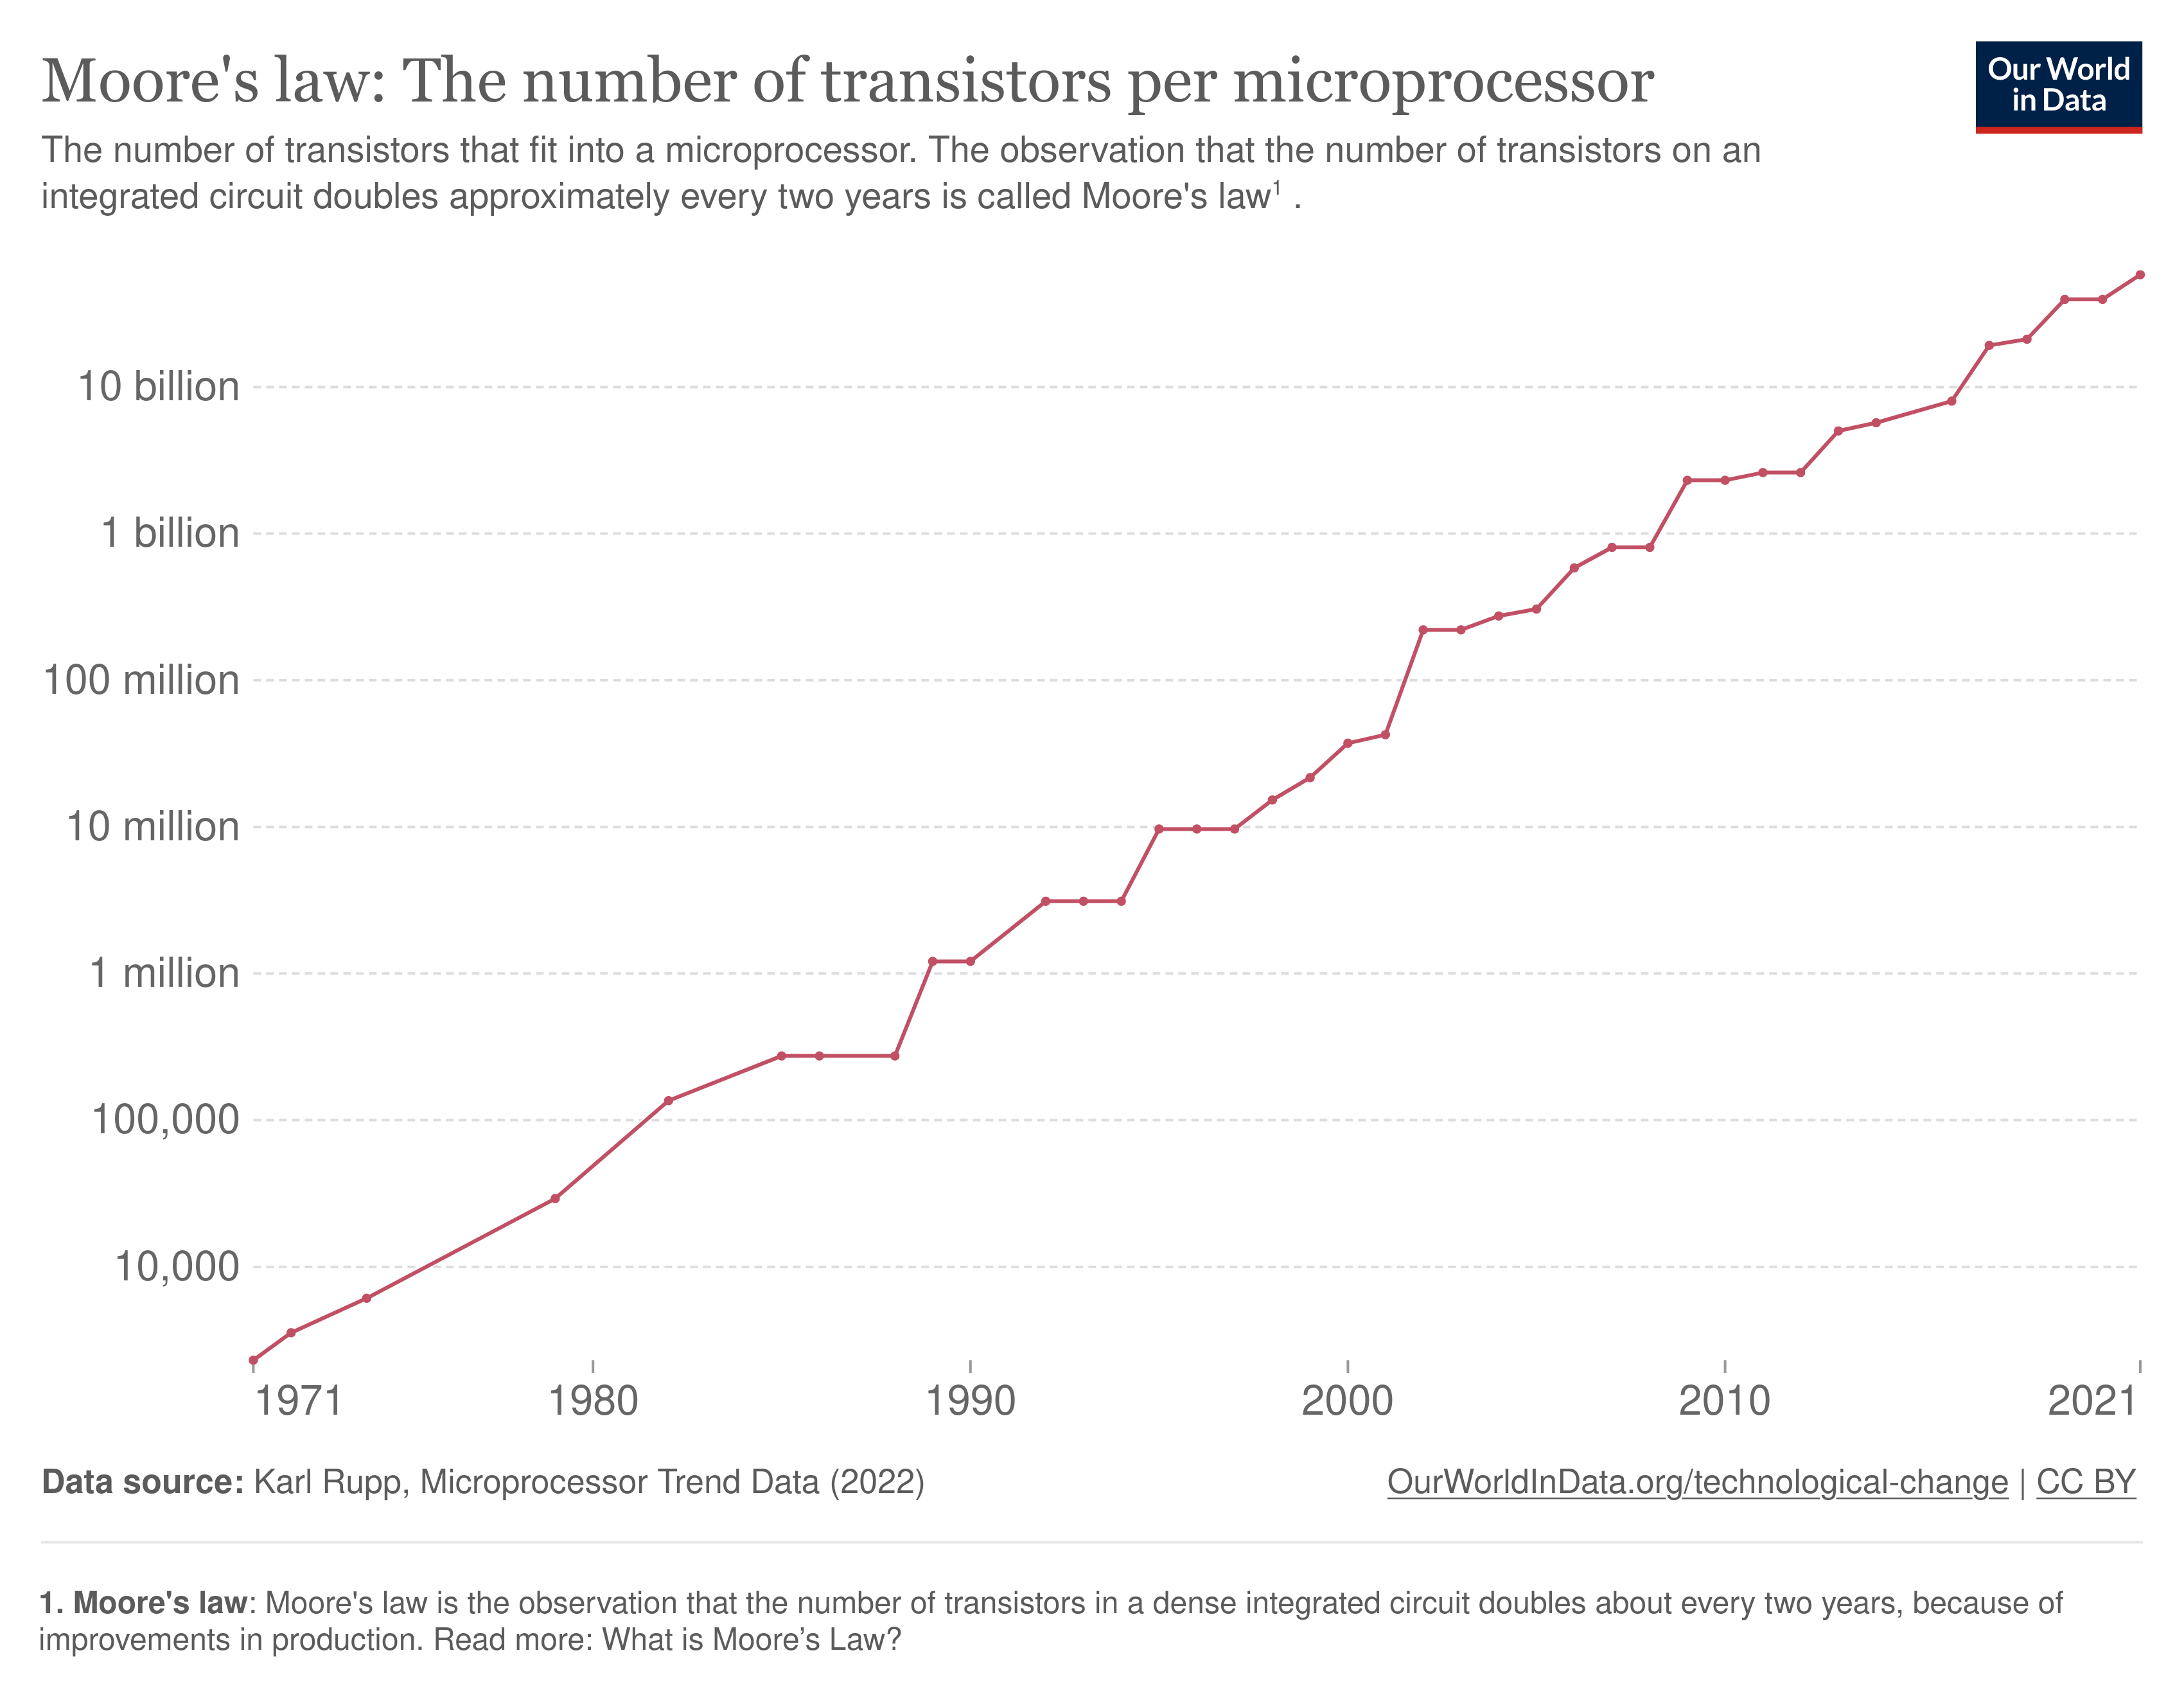
\includegraphics[width=.9\linewidth]{images/chapter1/moore_law2.png}
\caption{Legge di Moore}
\label{fig:moore_law}
\end{figure}

% GPU

Le \gls{GPU} sono speciali processori, che prendono a piene mani il concetto di multi-core e lo porta all'estremo, al punto da avere tantissimi core, più semplici e lenti dei core di una CPU, ma con un più alto throughput totale. 
Originariamente le GPU sono state sviluppate per scopi legati all'elaborazione grafica, in particolare, per migliorare la resa delle immagini e la grafica 3D nei videogiochi, nelle applicazioni \gls{CAD} e nei software di modellazione e rendering. In seguito, le esigenze di una grafica sempre più dettagliata e complessa ha portato alla creazione di unità di elaborazione specializzate con un'architettura che le rende energicamente più efficienti di una CPU, per algoritmi che processano grossi blocchi di dati in parallelo. Le GPU sono state quindi fruttate anche per scopi diversi dall'elaborazione grafica. Si sono rivelate particolarmente utili per applicazioni scientifiche, \gls{HPC} e tecniche che richiedono elaborazione intensive, come la simulazione di modelli numerici, l'analisi dei dati e il calcolo scientifico. Adesso, in particolare, le GPU sono particolarmente adatte per l'addestramento e l'esecuzione di reti neurali, diventando uno strumento fondamentale per lo sviluppo dell'intelligenza artificiale.

% GPGPU

Quando si parla di \gls{GPGPU} si intende l'utilizzo delle GPU per compiti di calcolo generale, rendendole molto più che semplici dispositivi per l'elaborazione grafica. Questo è fondamentale per accelerare algoritmi di calcolo che richiedono enorme quantità di risorse, a patto che la computazione sia parallelizzabile su più processori.
Calcoli che prima richiedevano l'uso di supercomputer, per essere eseguiti, adesso si possono eseguire con una normale GPU desktop. 
Nel 2011 secondo la lista Top500, che classifica e descrive nel dettaglio i 500 sistemi informatici non distribuiti più potenti al mondo, il Tianhe-1A risultava il secondo supercomputer più potente al mondo. Grazie a un sistema basato sulle GPU NVIDIA Tesla M2050 \cite[]{Tianhe-1A:link} il Tianhe-1A è riuscito a raggiungere i 4.7 petaFLOPS di potenza computazionale. Solamente un anno dopo, invece, in vetta alla classifica spiccava il Titan \cite[]{Titan:link} con un sistema basato sulle più recenti e performanti GPU Nvida Tesla K20X raggiungendo i 17.59 petaFLOPS di potenza.
Da quell'anno divenne chiaro che le GPU sarebbero diventate un componente essenziale nell'HPC tanto quanto lo erano nel desktop computing, e dato che il supercomputing è il motore trainante di molte delle tecnologie che vediamo nei processori moderni, si è venuto a creare un circolo virtuoso per cui la necessità di processori sempre più veloci per elaborare dataset sempre più grandi, ha porta l'industria a produrre supercomputer sempre più potenti. Ad oggi si sta delineando una divisione netta nella produzione di GPU per uso desktop e per uso scientifico, i principali produttori, quali AMD, NVIDIA (e più recentemente Intel) rilasciano prodotti specificatamente per l'uno o per l'altro segmento di mercato, con lo scopo di soddisfare i diversi requisiti di ogni settore. Da giugno 2023 il supercomputer più veloce al mondo è il Frontier \cite[]{Frontier:link} con un sistema basato sulle GPU Radeon Instinct MI250X con cui riesce a raggiungere i 1.67 exaFLOPS, divenendo così il primo exacale supercomputer al mondo. Grazie all'uso delle GPU in ambito HPC si sta riuscendo a incrementare le performance dei supercomputer in modo esponenziale, come si evince dalla fig. \ref{fig:supercomputer_flops}. L'incremento così repentino delle performance ha portato gli esperti di settore a scoprire una nuova legge empirica: la legge di Huang \cite[]{Huang:law}, da Jensen Huang, CEO e co-founder di NVIDIA. La legge, enuncia che le performance delle GPU `più che raddoppiano ogni due anni', in pratica, si tratta quindi di un'analoga della legge di Moore, ma applicata alle GPU.

\begin{figure}[ht]
\centering
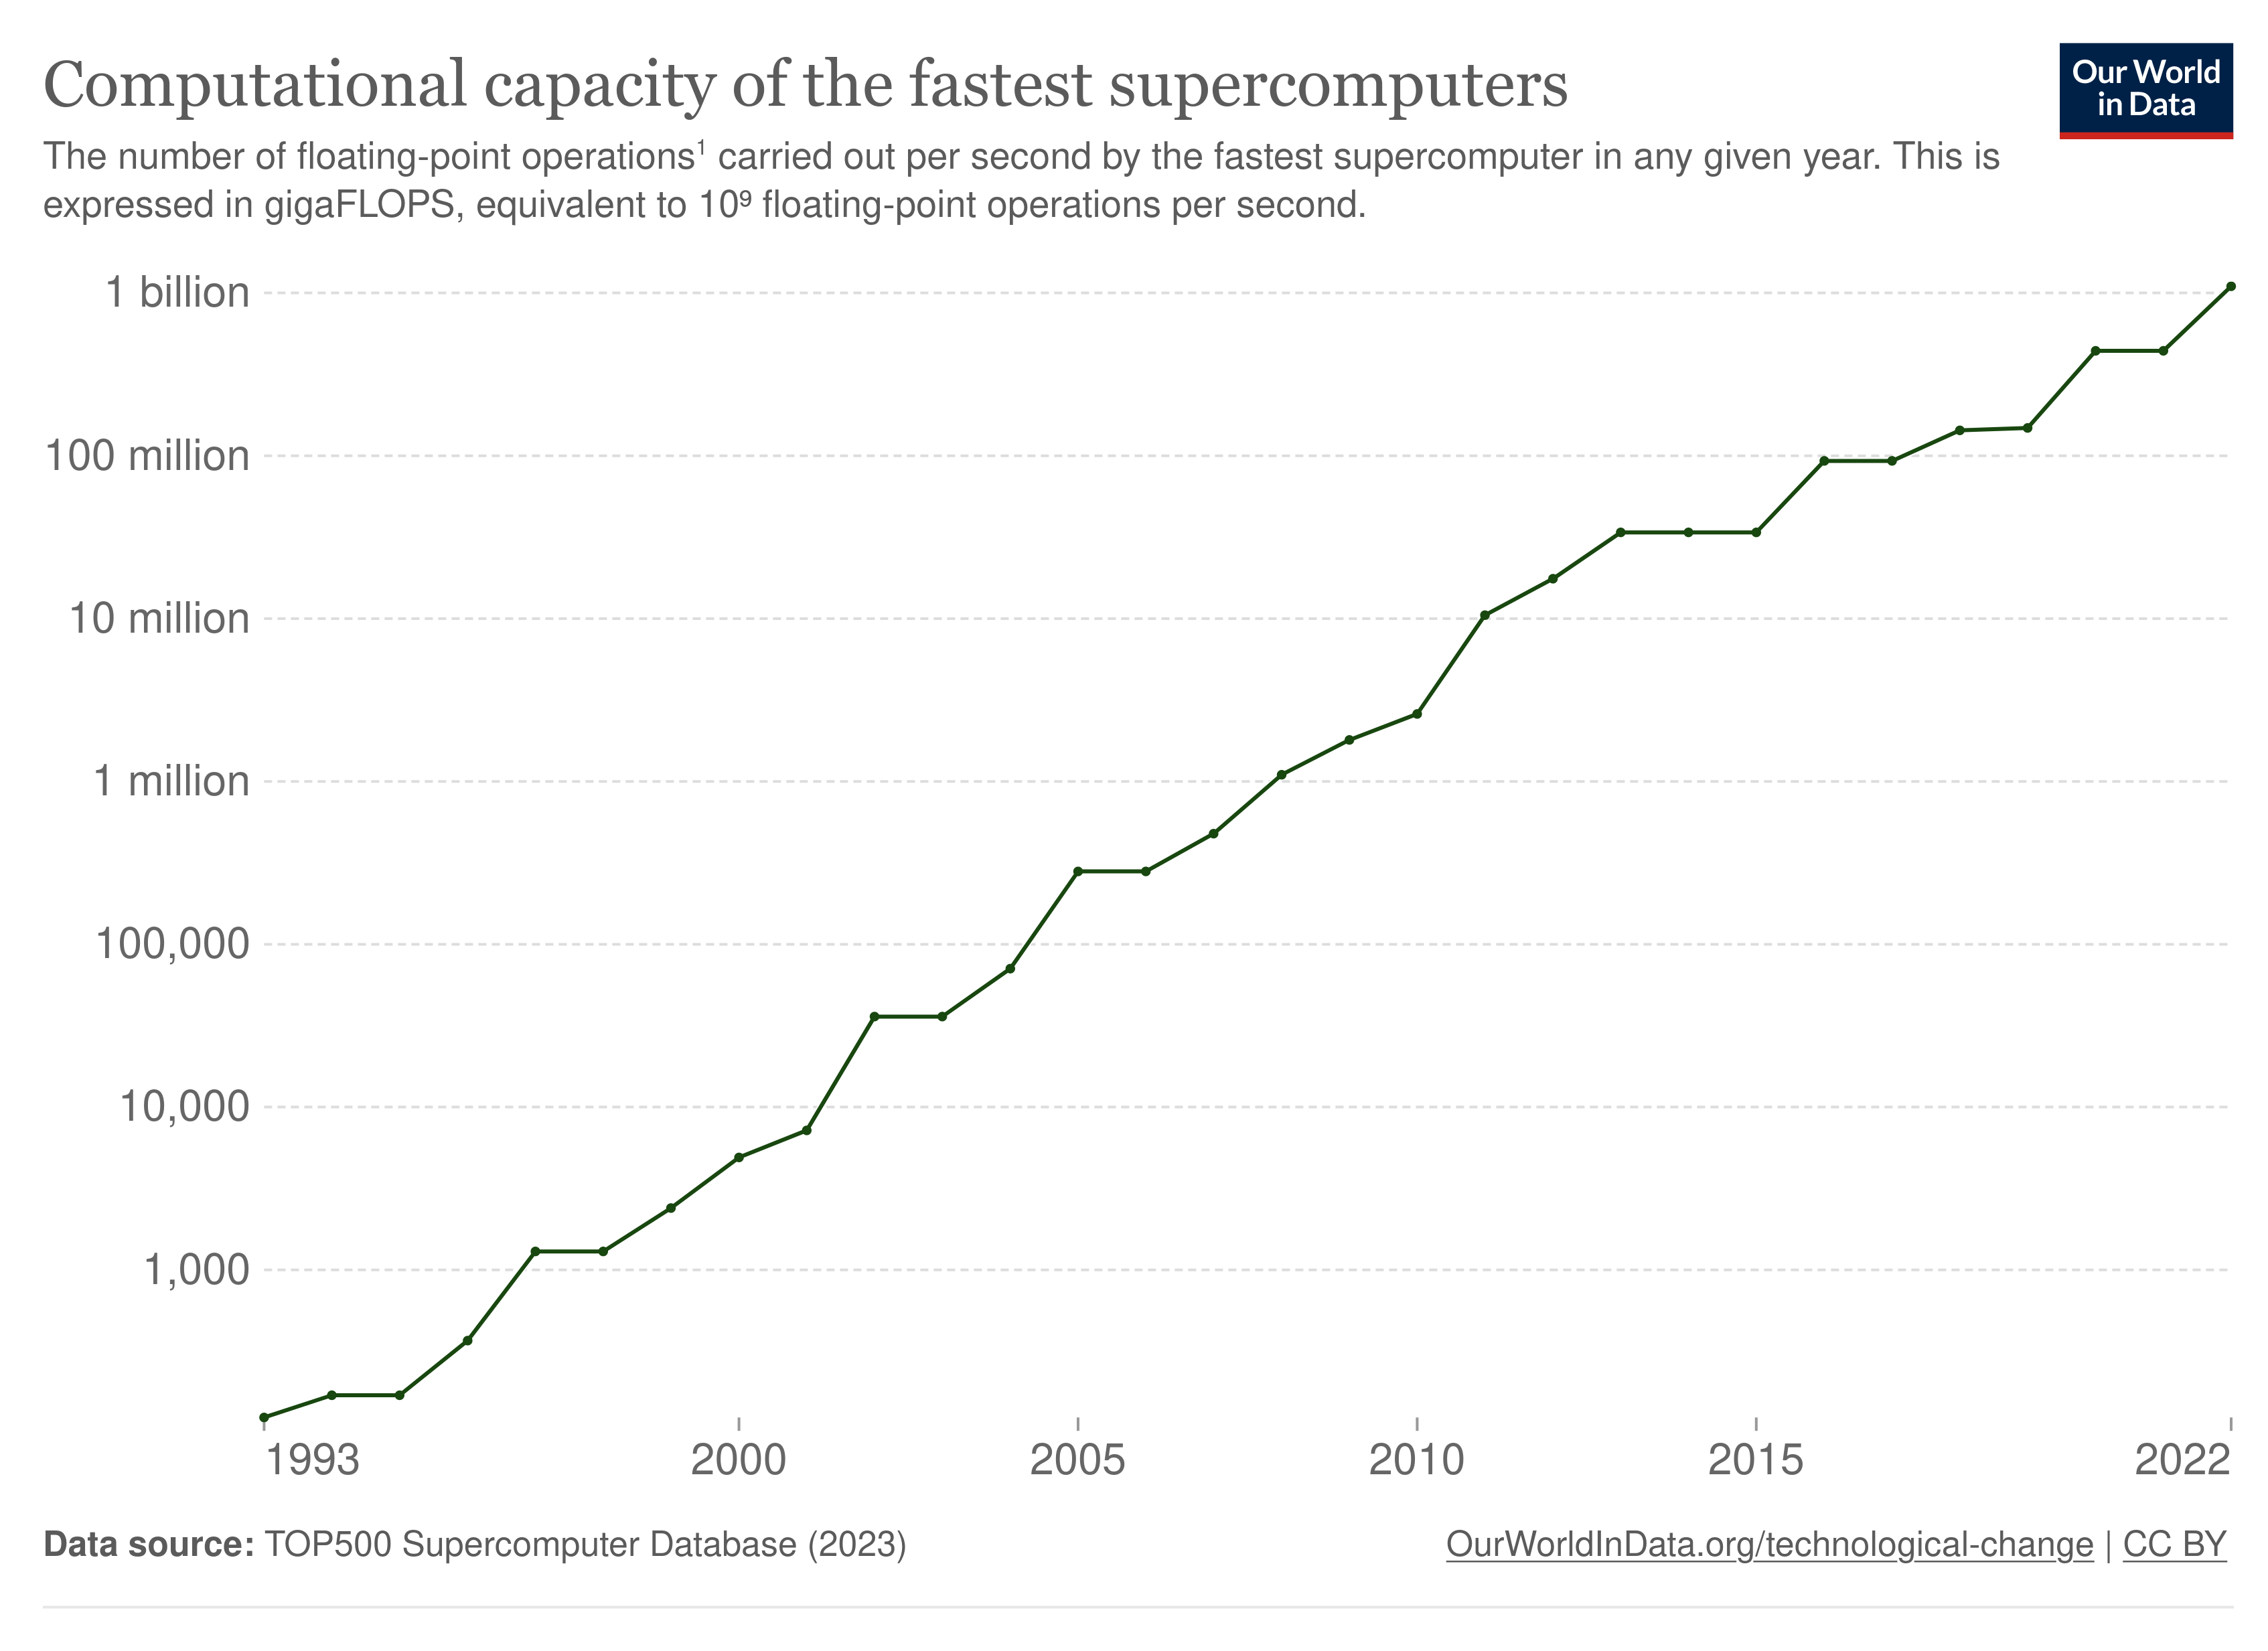
\includegraphics[width=.9\linewidth]{images/chapter1/supercomputer_flops.png}
\caption{Potenza dei supercomputer negli anni}
\label{fig:supercomputer_flops}
\end{figure}

%% Librerie GPU programming

Per poter programmare le GPU è stato necessario sviluppare delle \gls{API} che garantissero l'esecuzione del programma senza un'esplicita conversione dei dati in formato grafico. Le API oggi più utilizzate sono le \gls{CUDA} API di NVIDIA \cite[]{NVIDIA:CUDA} e le OpenCL API di Khronos Group \cite[]{KG:OpenCL}. Le API CUDA sfruttano l'omonima architettura delle GPU NVIDIA e sono in formato proprietario, mentre le API OpenCL, come suggerisce il nome, sono uno standard aperto royalty-free e supportano la maggior parte delle architetture GPU esistenti. Sebbene queste abbiano prestazioni di molto inferiori rispetto a CUDA, OpenCL è la prima scelta per lo sviluppo di applicazioni multi-piattaforma, proprio per la sua natura open e l'ampia gamma di hardware supportato. Nel 2015 Khronos Group annuncia le Vulkan API \cite[]{KG:Vulkan} e il formato SPIR-V \cite[]{KG:SPIR-V}. Vulkan è una API grafica e di calcolo che offre un accesso ad alta efficienza e multi-piattaforma alle GPU moderne, utilizzate in una vasta gamma di dispositivi, da PC e console ai telefoni cellulari e alle piattaforme embedded. Vulkan è stato progettato per sfruttare pesantemente il multithreading, permettendo la generazione di carichi di lavoro asincroni da parte di thread multipli della CPU, che eseguono il codice sulla GPU solo dopo una esplicita sottomissione. Inoltre, la sua natura `close-to-metal' permette un controllo oculato delle risorse della GPU: lo sviluppatore è responsabile della sincronizzazione, allocazione di memoria e della sottomissione del lavoro, avendo così minor overhead del driver rispetto ad approcci come CUDA e OpenCL. SPIR-V è un formato intermedio per shader e kernel, che permette di scrivere il codice una volta e compilarlo per diverse architetture, sia GPU che CPU. Vulkan e SPIR-V sono stati sviluppati per essere usati insieme, ma non sono strettamente legati, infatti SPIR-V può essere usato anche con OpenCL e OpenGL.

\section[Problema e Contributi]{Problema e Contributi}

% cspell:ignore Vulkan CUDA
L'obiettivo di questo lavoro di tesi è valutare i potenziali vantaggi derivanti dall'utilizzo di Vulkan e Rust per lo sviluppo di applicazioni di computing, rispetto all'approccio tradizionale basato su CUDA.
Nonostante Vulkan sia largamente usato nell'industria dei videogiochi, usarlo in ambito computing è una sfida non banale, a causa delle API verbose e del controllo meticoloso sulle strutture dati. 
Un'idea per ridurre il carico intellettivo per lo sviluppatore, e rendere la \textit{development experience} più appagante, può essere quella di optare per una gestione della memoria automatica. Solitamente quando si parla di gestione automatica della memoria si fa riferimento a garbage collector o contatori di riferimenti, per quanto valido possa essere questo approccio, il risultato non sempre è performante e ad alta efficienza, requisito fondamentale in questo ambito. Per mantenere le prestazioni quanto più vicine possibile a un'implementazione `low level', senza sacrificare l'ergonomicità di un approccio ad alto livello, si è scelto di coniugare i vantaggi del linguaggio Rust, quali, appunto, la gestione automatica della memoria senza strumenti di garbage collections, con quelli che offre Vulkan. 

Per poter capire se Vulkan e Rust sono una valida alternativa a CUDA per il computing, è necessario rispondere alle seguenti domande:

% bullet points
\begin{itemize}
    \item Qual è il livello di performance che Vulkan riesce a raggiungere rispetto a CUDA? 
    \item Quanto è difficile sviluppare un'applicazione per il computing in Vulkan?
    \item In un ambiente a microservizi, quanto è facile sviluppare e mantenere un'applicazione Vulkan scritta in Rust? 
    \item Qual è il livello di maturità dell'ecosistema Vulkan? E quello di Rust?
\end{itemize}

Per rispondere a queste domande si è agito nel seguente modo:

\begin{itemize}
    \item Si è scelto di implementare algoritmi altamente parallelizzabili su GPU, quali la somma di vettori e moltiplicazione di matrici, da usare come banco di prova per comparare le performance di due medesime implementazioni in CUDA e Vulkan, in particolare è preso in considerazione sia il tempo dell'esecuzione `pura' dell'algoritmo, che del trasferimento dei dati dalla memoria host (CPU) a quella device (GPU).
    \item Si è implementato gli algoritmi in Vulkan per valutare il potenziale delle sue API close-to-metal e quanto ergonomico sia sviluppare in Rust. Dato che sviluppare in Vulkan richiede degli step standard quali la creazione di un logical device, una pipeline, la compilazione del codice kernel e l'allocazione di memoria, si è usata la libreria Rust Vulkano \cite[]{Rust:Vulkano}, che implementa dei binding safe all'implementazione standard di Vulkan.
    \item Si è poi reimplementato i medesimi algoritmi in CUDA per comparare sia le performance che il diverso approccio alla scrittura dei kernel come estensione del linguaggio C++ tramite il compilatore \gls{NVCC} \cite[]{NVIDIA:nvcc}, osservando che GLSL \cite[]{KG:GLSL} usato in Vulkan offre più funzioni orientate alla grafica che al computing.
    \item Infine, considerando le necessità aziendali e i risultati relativi ai benchmark ottenuti, si è sviluppato un microservizio `proof of concept' che coniuga i vantaggi di Rust in ambito web con quelli di CUDA in ambito computing. Si è inoltre valutato anche altri possibili approcci alla soluzione del problema.
\end{itemize}



\section[Struttura della tesi]{Struttura della tesi}

!! TODO quando finiti tutti i capitoli

Il lavoro è stato progettato, sviluppato e testato con il supporto del team di Quantum Computing di Data Reply con sede a Torino. 

